\clearpage
\section{Lösungskonzept}\label{sec:Loesungskonzept}
Zur Messung und Auswertung der Mesh-Netzwerke dient ein Testframework wie es in Abbildung \ref{fig:KonzeptschemaTestframework} schematisch dargestellt ist.

\begin{figure}[H]
	\centering
	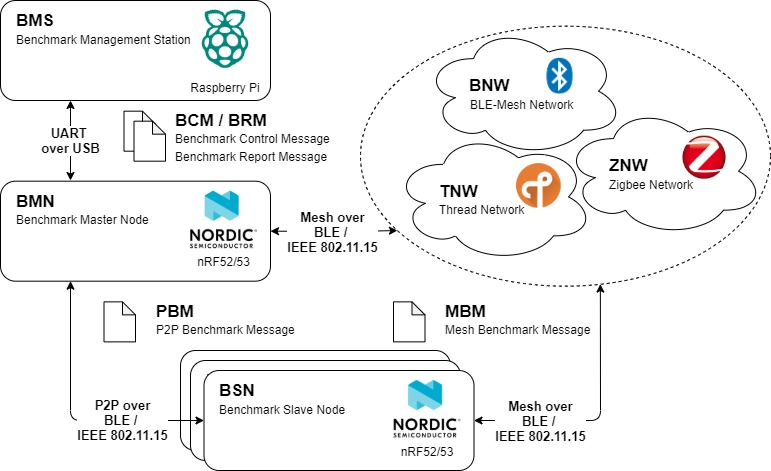
\includegraphics[width=1.0\textwidth]{Konzept_Testframework.jpg}
	\caption{Konzeptschema Testframework}\label{fig:KonzeptschemaTestframework}
\end{figure}


Das Testframework besteht aus folgenden physikalisch getrennten Teilsystemen:

\begin{itemize}
	\item \textbf{BMS} Benchmark Management Station \\ 
	Dient zur Verwaltung und Konfiguration des Testframeworks. Beinhaltet einen Webserver um dem Endanwender die Bedienung zu ermöglichen. Realisiert wird die BMS durch einen \textit{Raspberry Pi 4 Model B}. Als Webserver wird das Python-Framework \textit{Django} eingesetzt. 
	\item \textbf{BMN} Benchmark Master Node \\ 
	Dient als Zugangspunkt der BMS für die im Testframework gefahrenen Tests und lässt sich über eine Serielle Schnittstelle ansprechen. In der Aufgabenstellung \ref{app:Aufgabenstellung} wird der BMN als Master bezeichnet. Realisiert wird der BMN über einen nRF52840 oder nRF5340 von \textit{Nordic}. 
	\item \textbf{BSN} Benchmark Slave Node \\ 
	Dient als Zugriffspunkt der im Testframework gefahrenen Tests und kann frei in der Testumgebung platziert werden. Daher muss die Energieversorgung über einen Akku oder Batterie erfolgen. In der Aufgabenstellung  \ref{app:Aufgabenstellung} wird von einem Slave gesprochen. Realisiert wird der BSN über einen nRF52840 oder nRF5340 von \textit{Nordic}.
\end{itemize}

Die logischen Komponenten des Testframeworks lassen sich wie folgt aufteilen:

\begin{itemize}
	\item \textbf{BCM} Benchmark Control Message \\ 
	Beschreibt Nachrichten welche zur Steuerung eines Benchmarks dienen. Dies sind zum Beispiel Konfigurations-, Start- oder Stop-Befehle. Werden von der BMS initiiert und gelangen über eine USB-UART Verbindung zum BMN. 
	\item \textbf{BRM} Benchmark Report Message \\ 
	Beschreibt Nachrichten welche den Status oder die Ergebnisse eines Benchmarks zurückmelden. Werden vom BMN initiiert und gelangen über eine USB-UART Verbindung zur BMS.
	\item \textbf{PBM} P2P Benchmark Message \\ 
	Nachrichten welche während der Durchführung eines Benchmarks versendet werden. Dies sind zum Beispiel Ping-Anfragen zur Latenzzeitmessung. Sie ermöglichen den Datenaustausch zwischen zwei Teilnehmern auf MAC-Ebene. 
	\item \textbf{MBM} Mesh Benchmark Message \\ 
	Nachrichten welche während der Durchführung eines Benchmarks versendet werden. Dies sind zum Beispiel Ping-Anfragen zur Latenzzeitmessung. Sie ermöglichen den Datenaustausch über ein Mesh-Netzwerk auf Applikations-Ebene. 
\end{itemize}

\subsection{Punkt zu Punkt Testinfrastruktur}\label{subsec:PunktzuPunktTestinfrastruktur}

Der Punkt zu Punkt Benchmark (P2P) soll unabhängig vom Mesh-Protokoll stattfinden. Damit soll es möglich sein die beiden MAC-Ebenen \textit{BLE} und \textit{IEEE802.11.15} zu vergleichen. Der nRF52840 sowie nRF5340 unterstützen das Arbeiten auf der MAC-Schicht. Zur Realisierung wird ein bereits bestehendes Beispiel (Radio-Example) aus der nRF Connect SDK genutzt.


\subsection{Test Mesh Netzwerke}\label{subsec:TestMeshNetzwerke}

Der Mesh-Benchmark soll die verschiedenen Mesh-Netzwerke möglichst identisch ausmessen. Dazu dient bei allen Mesh-Netzwerken die Applikations-Schicht. Ein Mesh Netzwerk wird zwischen dem BMN und den BSN aufgebaut. Dazu werden die einzelnen Nodes über die BMS mit der entsprechenden Firmware geladen und anschliessend im Raum verteilt. Das Laden ist zu Beginn über eine Kabelverbindung (UART) vorgesehen. Zu einem späteren Zeitpunkt soll dies drahtlos mithilfe eines Bootloaders möglich gemacht werden. 

\subsubsection{Bluetooth Mesh}\label{subsubsection:Bluetooth Mesh}

Die BLE-Mesh Firmware der Nodes werden aus Beispielen der nRF Connect SDK und Zephyr abgeleitet. Das Mesh-Demo Beispiel erlaubt es die essentiellen Netzwerk Parameter fix vorzugeben. Dadurch müssen die Nodes nicht mehr Provisioniert werden und sind sofort einsatzbereit.

\newpage
\subsubsection{Thread}\label{subsubsection:Thread} 
Die Abbildung \ref{fig:ThreadKonzept} zeigt das Framework des Openthread Netzwerkes auf. Die BMS kommuniziert via UART mit dem wpantund Protokoll von Google. Die Daten zum NCP, welcher auf dem BMN realisiert wird, werden mit Hilfe von Spinel übertragen. Der BMN sendet die erhaltenen Daten danach in das Thread Netzwerk.

\begin{figure}[H]
	\centering
	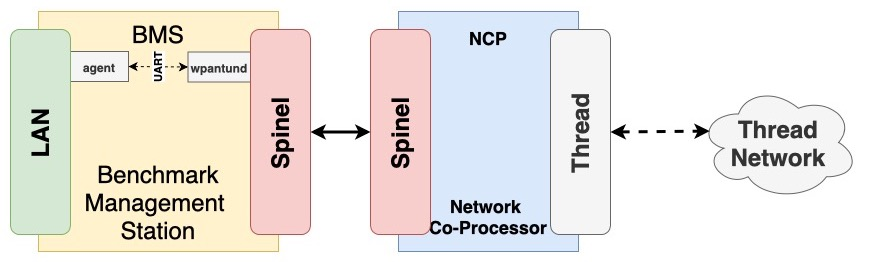
\includegraphics[width=1.0\textwidth]{Thread-Konzept.jpg}
	\caption{Konzept OpenThread Framework}\label{fig:ThreadKonzept}
\end{figure}



\subsubsection{Zigbee}\label{subsubsection:Zigbee}
Das Zigbee Test Mesh Netzwerk wird mithilfe der \textit{nRF SDK for Thread and Zigbee} eingerichtet und für die Messungen vorbereitet. Der BMN wird dabei als Zigbee Coordinator und gleichzeitig als Zigbee Router eingesetzt. Die BSN können wieder als Router oder aber als Zigbee End Device betrieben werden.


\subsection{Steuer und Auswertesoftware}\label{subsec:SteuerundAuswertesoftware}
Die Steuerung des Testframeworks erfolgt über eine Weboberfläche. Diese wird von der BMS mittels WLAN auf den Benutzergeräten zur Anzeige gebracht. Als Webserver dient das Python-Framework \textit{Django}. Zur Steuerung der Benchmarks dienen Schrittketten, welche mit der Firmware auf dem BMN kommunizieren. Als letzter Schritt eines Benchmarks werden die Ergebnisse geloggt, nachbearbeitet und wiederum zur Anzeige gebracht.

